\chapter{Analysis}
\label{sec:analysis}

\section{Correctness}

When we run our simulations, we want to determine whether NTP can give
accurate bounds on each node’s uncertainty range to include the real
time. This is the key characteristic of NTP that allows our algorithm
to work correctly.

At each node, NTP has an estimate for the real time and an uncertainty
in that estimate. Clknetsim allows us to access that information, and
it allows us to know the real time of the system. All of this allows
us to know what the “safety buffer” is for each node in real time.

The safety buffer, $S(t)$,  for a particular node is defined as:

\[ S(t) =U(t) - | t - E(t)| \]

where $t$ is the real time, $U(t)$ is NTP’s uncertainty in the real
time estimate for that node, and E(t) is NTP’s estimate for what the
real time is. In simpler terms, the safety buffer tells us where NTP’s
error in what the real time is lies within its uncertainty range (see
figure~\ref{fig:safety-diag}. If the safety buffer is a positive
value, then the difference between NTP’s estimate and real time is
within its uncertainty range. If it is negative, then it’s error is
outside of its uncertainty range, meaning that NTP doesn’t function as
we would expect.

\begin{figure}[h]
  \caption{} %% because label requires that it follow a caption in a fig
  \label{fig:safety-diag}
  \centering
  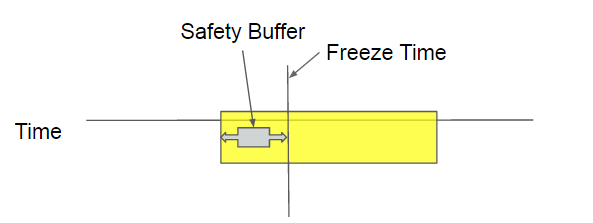
\includegraphics[width=0.8\textwidth]{safety-diagram.png}
\end{figure}

To prove the correctness of NTP, and therefore our algorithm, we ran a
Clknetsim simulation with 10 nodes over xxxxx %% TODO fill out your
section seconds, recording the safety buffer for each of the nodes at
every moment in time. We then aggregated those values for all of the
nodes together and we computed five points of data: the minimum value,
the maximum value, the average value, the average value plus one
standard deviation and the average value minus one standard
deviation. Those values are shown in figure~\ref{fig:safety-data}

\begin{figure}[h]
  \caption{}
  \label{fig:safety-data}
  \centering
  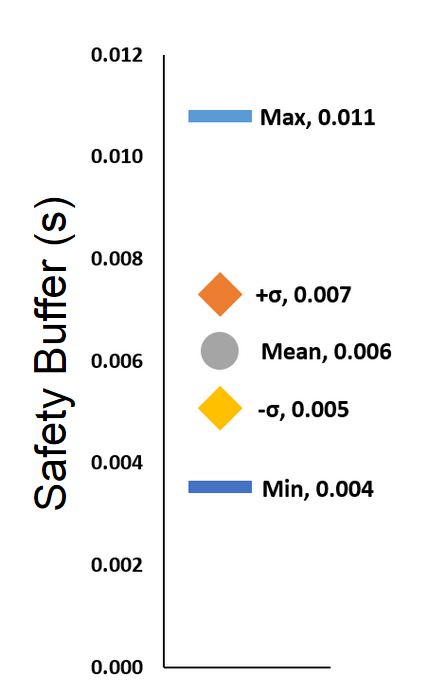
\includegraphics[width=0.8\textwidth]{safety-data.png}
\end{figure}

We can see that all of these values are positive. Since the minimum
value is a positive number, we can be sure that all of the values are
positive, which shows that NTP is functioning as we would
hope. Therefore, our algorithm can use NTP as a time synchronization
protocol.

\section{Performance}

Our testing has shown that NTP is a capable and resilient
algorithm. It seems likely that in any real-world network
configuration (baring hardware failure) NTP will be able to report
accuracy statistics that will result in the correct performance of our
algorithm. However, more exacting network layouts will be necessary to
make our algorithm performant. The data displayed in this section
summarizes trends seen when varying a number of parameters in a
standard network setup. We find few surprises -- network latency is
the standout determining factor for how performant our algorithm will
be. Lower the mean network latency and you will be rewarded by a
fairly consistently linear drop in freeze times.

It’s worth discussing how the network latency is modeled for these
simulations. Network latency was modeled using a gamma distribution,
since the data from the test Ceph cluster seemed to suggest that
latency approximately followed such a model. We varied two parameters:
the mean value and the shaping parameter, or alpha.

The shaping parameter represents how much of a tail our gamma
distribution has: a larger shaping parameter means that our gamma
distribution would have less of a tail. In the extremes, a small
shaping parameter approximates an exponential distribution and a large
shaping parameter approximates a normal distribution.

%% TODO please \ref these somewhere


\begin{figure}[h]
  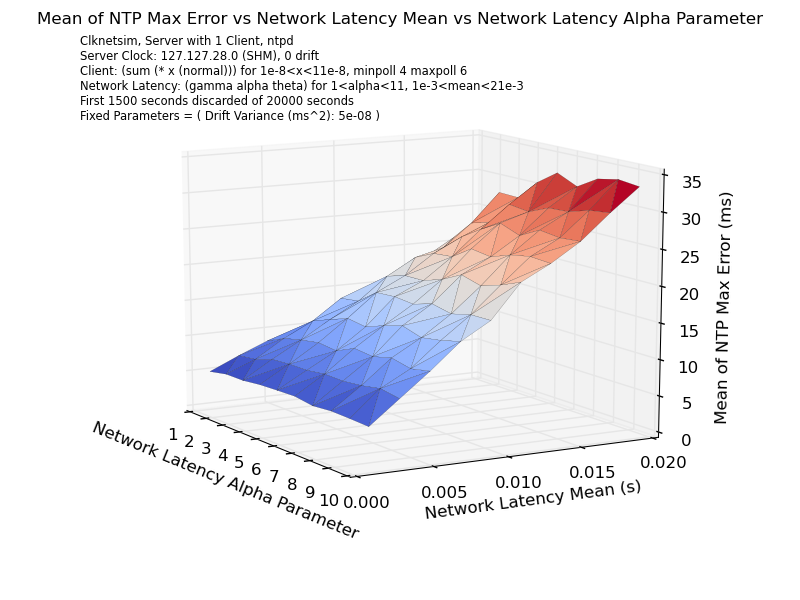
\includegraphics[width=1\linewidth]{mean_max_error-mean_latency-latency_alpha.png}
\end{figure}


\begin{figure}[h]
  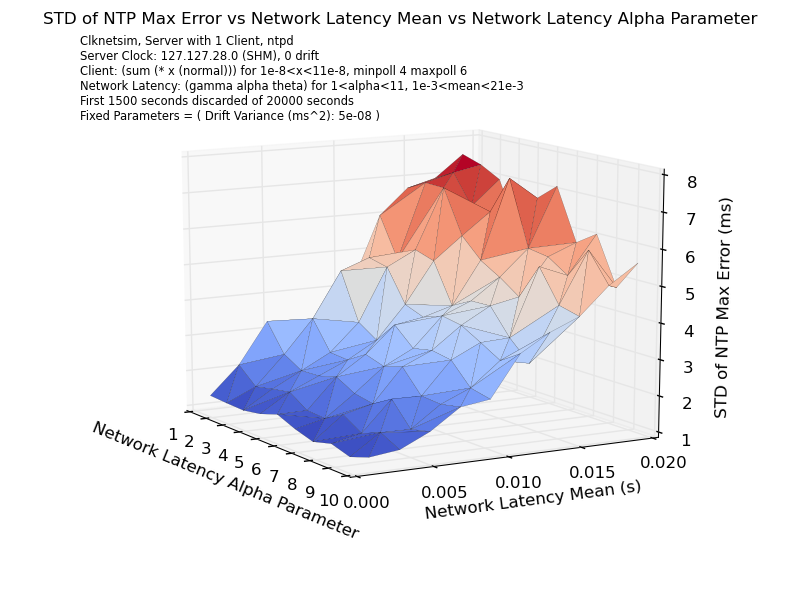
\includegraphics[width=1\linewidth]{max_err_stddev-latency_mean-latency_alpha.png}
\end{figure}

\begin{figure}[h]
  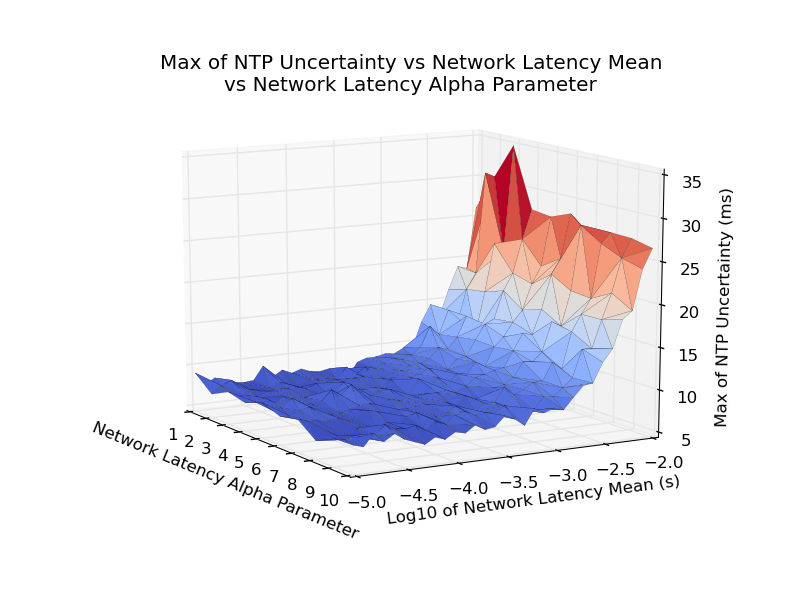
\includegraphics[width=1\linewidth]{max_error-latency_mean-latency_alpha.png}
\end{figure}

The NTP Max Error term is strongly affected by the mean network
latency. There is a much weaker effect on the Max Error by the shape
of the distribution of network latency traffic. NTP cares very little
about how the network tragic is distributed as long as the mean is
low. We can see in the upper right of MaxError vs Latency Mean vs
Alpha that there is a slight increase in Max Error for more
distributed latencies, especially as the mean latency grows.

Interestingly, we see that the mean of the max error term increases
with increasing alpha. This is likely because as alpha increases the
data become more normal. When the network latency distribution has a
long tail, most of our values will be less than or below the mean
value. Values larger and farther away from the mean tend to happen
less frequently and are more anomalous. Likely, NTP sees these values
are anomalies and ignores them, keeping its uncertainty at a lower,
more reasonable value. This explains why, for the graphs of the mean
and maximum of the error, we see lower values for lower alpha values.

As can be seen in figure~\ref{fig:max-mean-var-drift},
figure~\ref{fig:mean-mean-var-drift}, and
figure~\ref{fig:stddev-mean-drift-var} there is very little, if any,
effect of the drift variance of a node’s internal clock on the max
error term. This is expected network latency is a much larger term in
comparison to even the worst clocks. We again do see a strong,
apparently linear, correlation between mean latency and the max error
term. Looking at the mean of the max error term, we see values of
between 15 and 45 ms approximately. The max of the max error term for
any given run appears to be fairly predictable with few outliers in
the 20 to 70 ms range. The standard deviation of the measured max
error values is consistent with this, showing generally low
variability in the spread of max error values. We notice that the
spread does increase with increasing latency mean.

\begin{figure}[h]
  \caption{}
  \label{fig:max-mean-var-drift}
  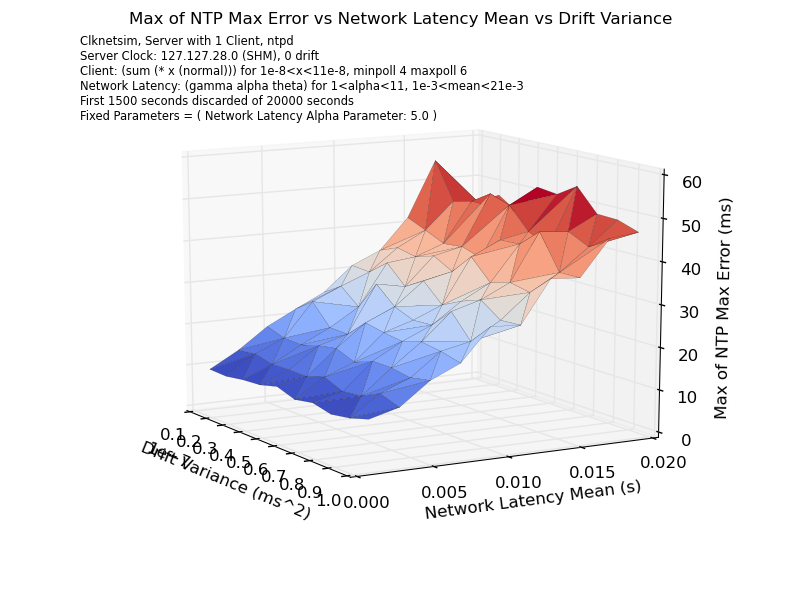
\includegraphics[width=1\linewidth]{max_max_err-mean_latency-drift_variance.png}
\end{figure}

\begin{figure}[h]
  \caption{}
  \label{fig:mean-mean-var-drift}
  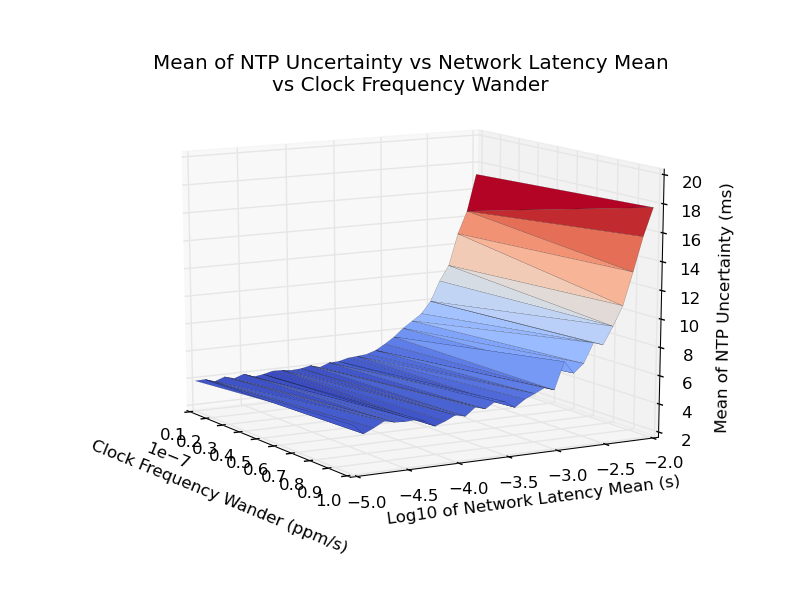
\includegraphics[width=1\linewidth]{mean_max_err-mean_latency-drift_variance.png}
\end{figure}

\begin{figure}[h]
  \caption{}
  \label{fig:stddev-mean-drift-var}
  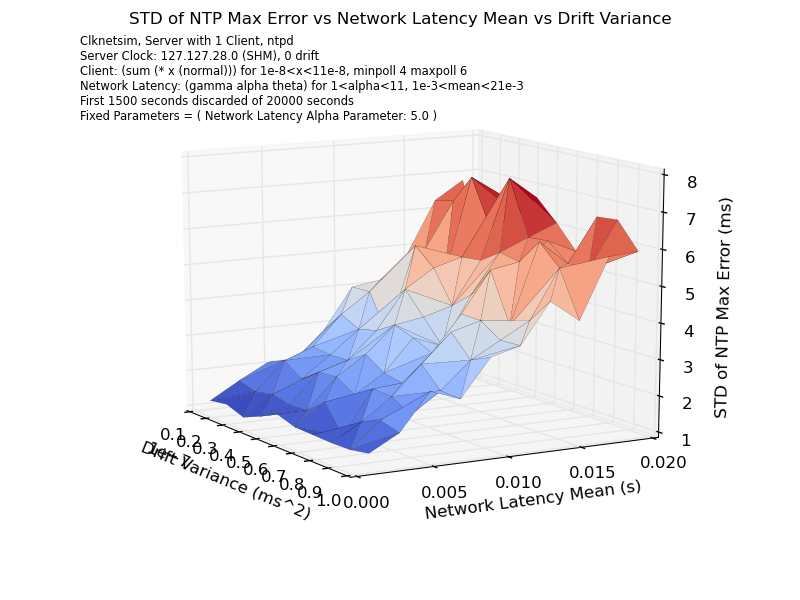
\includegraphics[width=1\linewidth]{stddev_max_err-mean_latency-drift_variance}
\end{figure}

Larger latency values do seem to mean that at any given time the
absolute time offset may be larger. However, network latency does not
seem to play a large role in the mean time offset. Drift seems to play
almost no role.

%% TODO please \ref these somewhere

\begin{figure}[h]
  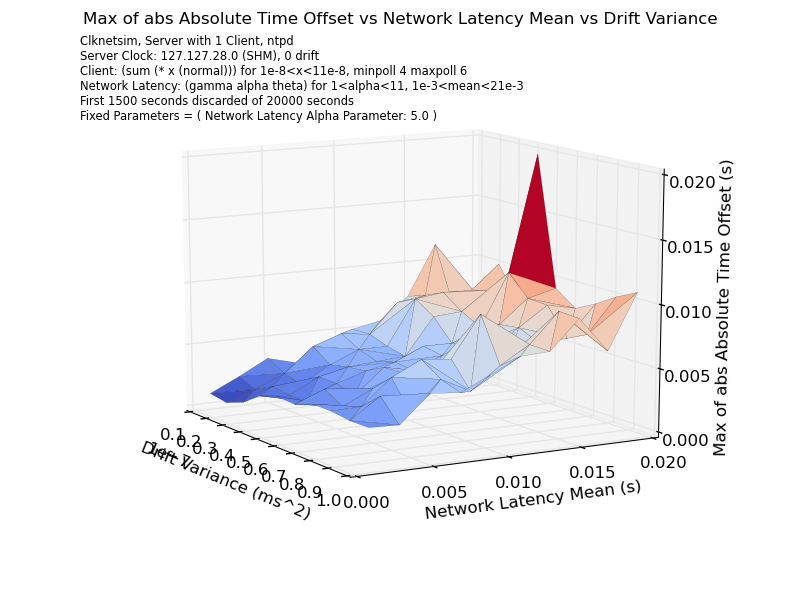
\includegraphics[width=1\linewidth]{max_abs_time-latency_mean-drift_var.png}
\end{figure}

\begin{figure}[h]
  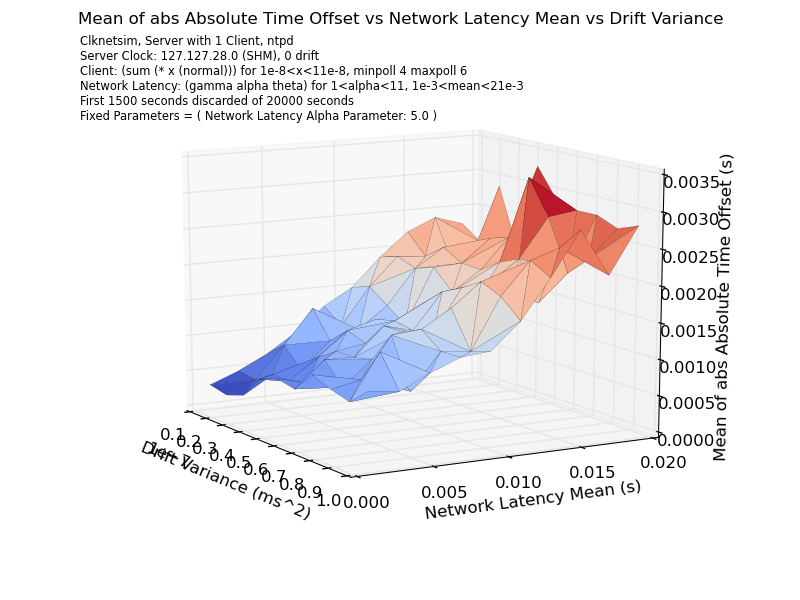
\includegraphics[width=1\linewidth]{mean_abs_time-mean_latency-drift_var.png}
\end{figure}

Larger latency values do seem to mean that at any given time the
absolute time offset may be larger. However, network latency does not
seem to play a large role in the mean time offset. Drift seems to play
almost no role.


%% TODO please \ref these somewhere

\begin{figure}[h]
  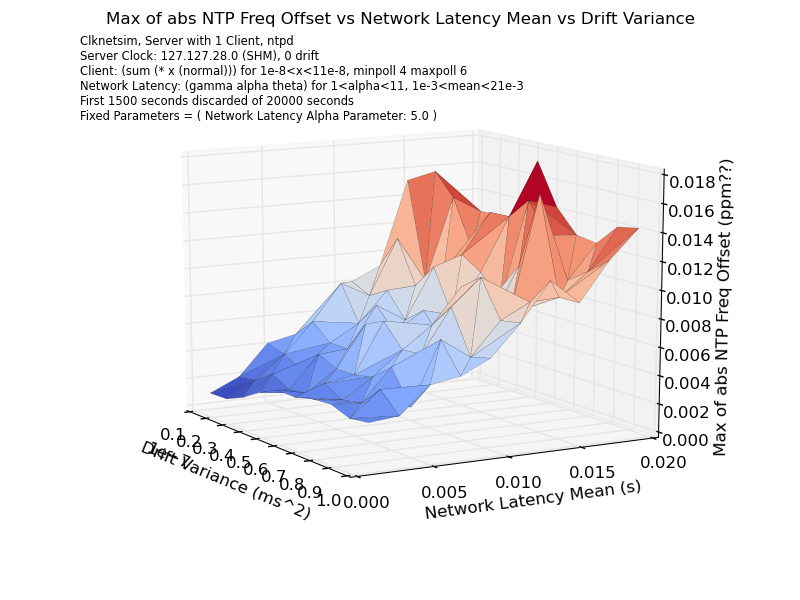
\includegraphics[width=1\linewidth]{max_abs_freq-mean_latency-drift_var.png}
\end{figure}

\begin{figure}[h]
  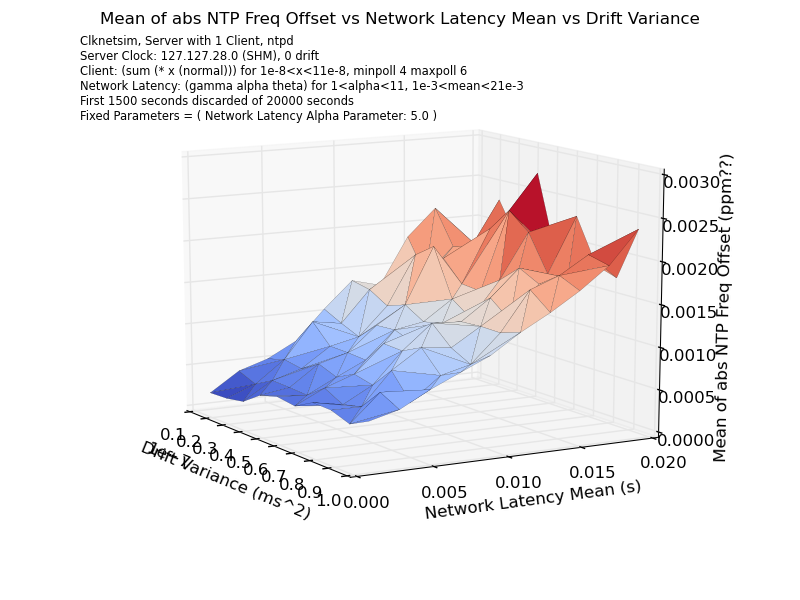
\includegraphics[width=1\linewidth]{mean_abs_freq-mean_latency-drift_var.png}
\end{figure}

\begin{figure}[h]
  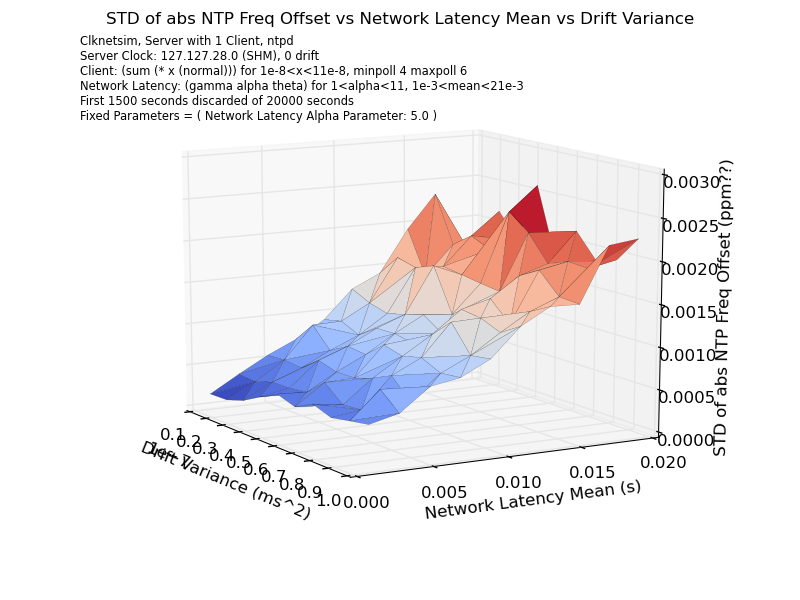
\includegraphics[width=1\linewidth]{stddev_abs_freq-mean_latency-drift_var.png}
\end{figure}

For larger variance in the drift, NTP does have to make larger
frequency corrections, but it seems that NTP is more than capable of
doing this as these clock discipline corrections do not seem to
translate into larger error or larger absolute time offsets. As the
mean latency increases, NTP also seems to make larger frequency
corrections. This likely means that, due to network asymmetries, NTP
is more likely to over correct or undercorrect at times, resulting in
an increase in the maximum offset. We also see that more normal
latency distributions also result is smaller deviations in the
frequency offset. The mean seems to not be significantly affected by
either the latency or the drift variance, suggesting that most of the
the clock frequency changes are the result of overcorrection and not
the result of the clock actually keeping poor time.

In summary, network latency mean has a larger effect on freeze
times. Network traffic shape does have an effect on freeze times, but
its effect is small in comparison to mean latency. An individual
node’s clock’s drift variance is inconsequential to the final
performance of our algorithm.

Due to how uncertainties compound in NTP, it is highly advisable to
acquire a single, good clock to serve as a master. This will
significantly decrease freeze windows.

